% Minimal preamble for Open Logic Project sources (pinned commit 1e960beff9ed7835bf3e3f1335e21af3439cd107).
%
% OLP's own master preamble cannot run on the project host: TeX Live 2025 there lacks
% prooftree.sty, ntheorem.sty, extarrows.sty, mathdots.sty, isomath.sty and subfiles.sty.
% Following the project's own rule ("if the author preamble needs packages the toolchain lacks,
% do not invent macros -- use a minimal working preamble"), this file declares, verbatim in
% spirit and numbering behaviour, exactly the theorem-like environments OLP defines in
% sty/open-logic-book-envs.sty (thm/lem/prop/cor/defn/ex/prob/rem/note/case/axiom/conv),
% plus the shorthand accents OLP uses (`!!a`, `!!b`, `!!{...}`).
%
% Author text is untouched; only the packaging is ours.
\documentclass[10pt,a4paper]{article}

\usepackage{amsmath}
\usepackage{amssymb}
\usepackage{amsthm}
\usepackage{graphicx}
\usepackage{hyperref}
\usepackage{enumitem}
\usepackage[framemethod=default]{mdframed}

% ---- OLP shorthand accents (from sty/open-logic.sty) ----
% NB: \! is taken by LaTeX (negative thin space), so we only define the !!a / !!b families
% and the \olup helper used by them.
\newcommand*{\olup}[1]{\MakeUppercase{#1}}
\def\!!!a#1{\olup{#1}}
\def\!!a#1{\olup{#1}}
\def\!!b#1{\olup{#1}}

% ---- theorem-like environments, same family numbering as OLP ----
\theoremstyle{plain}
\newtheorem{thm}{Theorem}[section]
\newtheorem{lem}[thm]{Lemma}
\newtheorem{prop}[thm]{Proposition}
\newtheorem{cor}[thm]{Corollary}
\newtheorem{axiom}{Axiom}

\theoremstyle{definition}
\newtheorem{defn}[thm]{Definition}
\newtheorem{ex}[thm]{Example}
\newtheorem{prob}{Problem}[section]
\newtheorem{probd}{Problem}
\newtheorem{conv}[thm]{Convention}

\theoremstyle{remark}
\newtheorem{rem}[thm]{Remark}
\newtheorem{note}[thm]{Note}
\newtheorem{case}[thm]{Case}

% ---- environments OLP defines as wrappers ----
\newenvironment{probtag}[1]{\begin{prob}}{\end{prob}}
\newenvironment{explain}{}{}
\newenvironment{explain*}{}{}
\newenvironment{editorial}{}{}
\newenvironment{digress}{}{}
\newenvironment{digress*}{}{}
\newenvironment{history}{}{}
\newenvironment{reference}{}{}
\newcommand*{\olfileid}[3]{}
\newcommand*{\olsection}[1]{\section*{#1}}
\newcommand*{\olchapter}[3]{}
\newcommand*{\olpart}[2]{}
\newcommand*{\olimport}[1]{}
\newcommand*{\olinclude}[1]{}
\newcommand*{\olpath}[1]{}
\newcommand*{\ollangid}[1]{}
\newcommand*{\problemtag}[1]{}
\newcommand*{\problemauthor}[1]{}
\newcommand*{\ollabel}[1]{\label{#1}}
% \olref takes 0-3 OPTIONAL arguments plus one mandatory label:
%     \olref{lab}  |  \olref[from]{lab}  |  \olref[from][to]{lab}  |  \olref[a][b][c]{lab}
% A single-argument definition silently swallows "[sth]" and emits a broken reference
% (measured on the host: the text came out as "??iso]x"). The chain below consumes the
% brackets and cross-references only the mandatory argument.
\makeatletter
\newcommand{\olref}{\@ifnextchar[{\olref@i}{\olref@final}}
\def\olref@i[#1]{\@ifnextchar[{\olref@ii}{\olref@final}}
\def\olref@ii[#1]{\@ifnextchar[{\olref@iii}{\olref@final}}
\def\olref@iii[#1]{\olref@final}
\def\olref@final#1{\ref{#1}}
\makeatother
\newcommand*{\olnewpage}{\clearpage}

% ===================== OLP compatibility layer (1) =====================

\makeatletter

% ---------------- proof trees (OLP's prooftree is a bussproofs derivative) ----------------
\providecommand{\AxiomC}[1]{}
\providecommand{\UnaryInfC}[1]{}
\providecommand{\BinaryInfC}[1]{}
\providecommand{\TrinaryInfC}[1]{}
\providecommand{\QuaternaryInfC}[1]{}
\providecommand{\QuinaryInfC}[1]{}
\providecommand{\RightLabel}[1]{}
\providecommand{\LeftLabel}[1]{}
\providecommand{\doubleLine}{}
\providecommand{\noLine}{}
\providecommand{\DisplayProof}{}
\providecommand{\fCenter}{}
\newenvironment{prooftree}{}{}
\newenvironment{ltprooftree}{}{}
\newenvironment{oltableau}{}{}

% ---------------- logical notation ----------------
\providecommand{\lif}{\mathbin{\rightarrow}}
\providecommand{\lforall}{\mathord{\forall}}
\providecommand{\lexists}{\mathord{\exists}}
\providecommand{\ltrue}{\top}
\providecommand{\lfalse}{\bot}
\providecommand{\Ltrue}{\top}
\providecommand{\Lfalse}{\bot}
\providecommand{\Sequent}{\mathrel{\Rightarrow}}
\providecommand{\Proves}{\mathrel{\vdash}}
\providecommand{\Entails}{\mathrel{\models}}
\providecommand{\Subst}[3]{#1[#2/#3]}
\providecommand{\sFmla}[2]{#1(#2)}
\providecommand{\pFmla}[2]{#1(#2)}
\providecommand{\formula}{\relax}
\providecommand{\True}{\top}
\providecommand{\False}{\bot}
\providecommand{\Args}[1]{#1}
\providecommand{\Ts}{\ensuremath{\top}}
\providecommand{\Fi}{\ensuremath{\bot}}
\providecommand{\lfalsum}{\bot}

% ---------------- objects, structures, metatheory ----------------
\providecommand{\Obj}{}
\providecommand{\Struct}{\ensuremath{\mathfrak{A}}}
\providecommand{\Domain}{\ensuremath{|\mathfrak{A}|}}
\providecommand{\Assign}{\ensuremath{s}}
\providecommand{\Sat}[2]{\ensuremath{#1 \models #2}}
\providecommand{\mSat}[3]{\ensuremath{#1 \models #2[#3]}}
\providecommand{\mModel}[2]{\ensuremath{#1 \models #2}}
\providecommand{\Lang}{\ensuremath{\mathcal{L}}}
\providecommand{\Th}{\ensuremath{\mathrm{Th}}}
\providecommand{\Log}{\ensuremath{\mathrm{L}}}
\providecommand{\tuple}[1]{\langle #1 \rangle}
\providecommand{\num}[1]{\underline{#1}}
\providecommand{\cfind}[1]{\varphi_{#1}}
\providecommand{\Nat}{\ensuremath{\mathbb{N}}}
\providecommand{\Mult}{\ensuremath{\mathrm{Mult}}}
\providecommand{\Add}{\ensuremath{\mathrm{Add}}}
\providecommand{\Exp}{\ensuremath{\mathrm{Exp}}}
\providecommand{\Zero}{\ensuremath{0}}
\providecommand{\Succ}{\ensuremath{\mathrm{S}}}
\providecommand{\lambd}{\ensuremath{\lambda}}
\providecommand{\bredpar}{\mathrel{\rightarrow_\beta}}
\providecommand{\bcd}[1]{\ensuremath{\ulcorner #1 \urcorner}}
\providecommand{\Set}[1]{\ensuremath{\{#1\}}}
\providecommand{\indcase}[1]{\par\noindent\emph{Case #1}.\quad}
\providecommand{\indfrm}[1]{\par\noindent\emph{Form #1}.\quad}
\providecommand{\iftag}[1]{#1}
\providecommand{\tagitem}[1]{\item[#1]}
\providecommand{\Elim}[1]{}
\providecommand{\Intro}[1]{}
\providecommand{\LeftR}[1]{}
\providecommand{\RightR}[1]{}
\providecommand{\TAss}[1]{}
\providecommand{\TRule}[1]{}

\makeatother
\providecommand{\olpath}{.}

% ===================== OLP compatibility layer (2) =====================
% --- second compatibility block: notation and shorthands used by the frozen OLP units ---
\providecommand{\CutCS}{\mathrm{Cut}}
\providecommand{\LeftSubproofLabel}{\relax}
\providecommand{\RightSubproofLabel}{\relax}
\providecommand{\maeh}{\relax}
\providecommand{\cheight}{\relax}
\providecommand{\ande}{\mathrm{and}_E}
\providecommand{\andi}{\mathrm{and}_I}
\providecommand{\ore}{\mathrm{or}_E}
\providecommand{\ori}{\mathrm{or}_I}
\providecommand{\typeof}{\mathord{:}}
\providecommand{\pValue}[1]{#1}
\providecommand{\Sent}{\mathrm{Sent}}
\providecommand{\cardplus}{\mathbin{+}}
\providecommand{\cardtimes}{\mathbin{\cdot}}
\providecommand{\cardexpo}{\mathbin{\hat{\ }}}
\providecommand{\cardnless}{\not<}
\providecommand{\cardle}{\leq}
\providecommand{\funfromto}[3]{#1\colon #2 \to #3}
\providecommand{\funimage}[1]{\operatorname{im}(#1)}
\providecommand{\fdefined}{\mathord{\downarrow}}
\providecommand{\canonord}{\operatorname{ord}}
\providecommand{\ordtimes}{\mathbin{\cdot}}
\providecommand{\ordeq}[2]{#1 = #2}
\providecommand{\ordneq}[2]{#1 \neq #2}
\providecommand{\ordtype}[1]{\operatorname{ord}(#1)}
\providecommand{\ordsucc}{\mathord{+1}}
\providecommand{\ordunion}{\cup}
\providecommand{\onesphere}{S^1}
\providecommand{\rotationsgroup}{\mathrm{SO}(2)}
\providecommand{\equivrep}[1]{[#1]}
\providecommand{\rlexless}{\prec}
\providecommand{\ZFC}{\mathrm{ZFC}}
\providecommand{\ZF}{\mathrm{ZF}}
\providecommand{\Rat}{\mathbb{Q}}
\providecommand{\Real}{\mathbb{R}}
\providecommand{\PosInt}{\mathbb{Z}^{+}}
\providecommand{\Id}{\mathrm{id}}
\providecommand{\Bin}{\mathrm{Bin}}
\providecommand{\pto}{\rightharpoonup}
\providecommand{\dom}{\operatorname{dom}}
\providecommand{\ran}{\operatorname{ran}}
\providecommand{\len}{\operatorname{len}}
\providecommand{\concat}{\mathbin{{}^\frown}}
\providecommand{\card}[1]{\lvert #1 \rvert}
\providecommand{\Pow}{\mathcal{P}}
\providecommand{\Setabs}[2]{\{\, #1 \mid #2 \,\}}
\providecommand{\comp}{\circ}
\providecommand{\Char}{\chi}
\providecommand{\Prf}{\operatorname{Prf}}
\providecommand{\Prov}{\operatorname{Prov}}
\providecommand{\Proj}{\operatorname{proj}}
\providecommand{\Gn}{\operatorname{gn}}
\providecommand{\gn}{\operatorname{gn}}
\providecommand{\Value}[1]{\operatorname{val}(#1)}
\providecommand{\Deduce}{\mathrm{D}}
\providecommand{\Dual}{\mathrm{d}}
\providecommand{\Ax}{\mathrm{Ax}}
\providecommand{\pSat}[3]{#1 \models #2\,[#3]}
\providecommand{\pAssign}{\sigma}
\providecommand{\bforall}{\forall}
\providecommand{\bexists}{\exists}
\providecommand{\liff}{\mathbin{\leftrightarrow}}
\providecommand{\FV}{\operatorname{FV}}
\providecommand{\UnaryInf}{\ensuremath{\mid}}
\providecommand{\BinaryInf}{\ensuremath{\mid}}
\providecommand{\depth}{\operatorname{depth}}
\providecommand{\oliflabeldef}[3]{#1}
\providecommand{\TMblank}{\sqcup}
\providecommand{\TMstroke}{\mid}
\providecommand{\TMstay}{\mathrm{S}}
\providecommand{\TMright}{\mathrm{R}}
\providecommand{\TMleft}{\mathrm{L}}
\providecommand{\TMendtape}{\triangleright}
\providecommand{\umin}{\mu}
\providecommand{\Sum}{\sum}
\providecommand{\citep}[1]{\cite{#1}}
\providecommand{\citet}[1]{\cite{#1}}
\providecommand{\citeauthor}[1]{\cite{#1}}
\providecommand{\citeyear}[1]{\cite{#1}}

% ===================== OLP compatibility layer (3) =====================
% --- third compatibility block: remaining notation seen in the frozen OLP units ---
\providecommand{\iso}{\cong}
\providecommand{\nszero}{\mathrm{0}}
\providecommand{\nssucc}{\mathrm{S}}
\providecommand{\nsplus}{\mathbin{+}}
\providecommand{\nssless}{<}
\providecommand{\nsless}{<}
\providecommand{\PL}{\mathrm{PL}}
\providecommand{\Nec}{\mathord{\Box}}
\providecommand{\RK}{\mathrm{RK}}
\providecommand{\ST}{\mathrm{ST}}
\providecommand{\SSubst}[3]{#1[#2/#3]}
\providecommand{\subst}[3]{#1[#2/#3]}
\providecommand{\tagfalse}{\mathrm{F}}
\providecommand{\cutr}{\mathrm{Cut}}
\providecommand{\cardneq}{\neq}
\providecommand{\issucc}[1]{\operatorname{succ}(#1)}
\providecommand{\tup}[1]{\langle #1 \rangle}
\providecommand{\Var}{\mathrm{Var}}
\providecommand{\Bew}{\operatorname{Bew}}
\providecommand{\Con}{\operatorname{Con}}
\providecommand{\Cons}{\operatorname{Cons}}
\providecommand{\pDeduce}{\mathrm{D}}
\providecommand{\psat}{\models}
\providecommand{\den}[1]{\llbracket #1 \rrbracket}
\providecommand{\Sem}[2]{\llbracket #1 \rrbracket_{#2}}
\providecommand{\DomainOf}[1]{\lvert #1 \rvert}
\providecommand{\Form}{\mathrm{Form}}
\providecommand{\Terms}{\mathrm{Term}}
\providecommand{\Atom}{\mathrm{Atom}}
\providecommand{\FVars}[1]{\operatorname{FV}(#1)}
\providecommand{\fv}[1]{\operatorname{fv}(#1)}
\providecommand{\tuplep}[1]{\langle #1 \rangle}
\providecommand{\restrict}[2]{#1 \upharpoonright #2}
\providecommand{\sto}{\rightarrow}
\providecommand{\FmlaSet}[1]{\mathrm{Fmla}_{#1}}
\providecommand{\Thm}{\mathrm{Thm}}
\providecommand{\Eval}{\operatorname{val}}
\providecommand{\blank}{\sqcup}
\providecommand{\blankTape}{\sqcup}
\providecommand{\Consis}{\operatorname{Con}}
\providecommand{\drs}{\mathrm{d}}
\providecommand{\VRule}{\mid}
\providecommand{\Bet}{\mathrm{B}}
\providecommand{\Seg}[1]{\mathrm{Seg}_{#1}}
\providecommand{\Enums}{\mathrm{En}}
\providecommand{\Z}{\mathbb{Z}}
\providecommand{\N}{\mathbb{N}}
\providecommand{\abs}[1]{\lvert #1 \rvert}
\providecommand{\floor}[1]{\lfloor #1 \rfloor}
\providecommand{\ceil}[1]{\lceil #1 \rceil}

% ===================== OLP compatibility layer (4) =====================
% --- fourth compatibility block: harvested from the per-candidate compile logs ---
\providecommand{\beredpar}{\mathrel{\rightarrow_\beta}}
\makeatletter
\def\bered{\@ifnextchar[{\bered@i}{\mathrel{\rightarrow_\beta}}}
\def\bered@i[#1]{\mathrel{\rightarrow_\beta}}
\def\bred{\@ifnextchar[{\bred@i}{\mathrel{\rightarrow_\beta}}}
\def\bred@i[#1]{\mathrel{\rightarrow_\beta}}
\makeatother
\providecommand{\beredone}{\mathrel{=_\beta}}
\providecommand{\bredone}{\mathrel{=_\beta}}
\providecommand{\xredone}{\mathrel{=_\beta}}
\providecommand{\aconvone}{\mathrel{=_\alpha}}
\providecommand{\cardless}{<}
\providecommand{\tagrefs}[1]{#1}
\providecommand{\ordplus}{\mathbin{+}}
\providecommand{\funrestrictionto}[2]{#1 \upharpoonright #2}
\providecommand{\fundefined}{\mathord{\uparrow}}
\providecommand{\Trm}{\mathrm{Trm}}
\providecommand{\OProv}{\operatorname{Prov}}
\providecommand{\OPrf}{\operatorname{Prf}}
\providecommand{\aeq}{\mathrel{=}}
\providecommand{\mClass}[1]{[#1]}
\providecommand{\equivclass}[1]{[#1]}
\providecommand{\pheight}{\operatorname{ht}}
\providecommand{\phy}{\operatorname{ht}}
\providecommand{\Cut}{\mathrm{Cut}}
\providecommand{\QuantRank}{\operatorname{qr}}
\providecommand{\elemequiv}{\mathrel{\equiv}}
\providecommand{\PIso}{\mathrm{PIso}}
\providecommand{\Theory}{\mathrm{Th}}
\providecommand{\supstrict}{\subsetneq}
\providecommand{\trcl}{\operatorname{trcl}}
\providecommand{\cref}[1]{\ref{#1}}
\providecommand{\Discharge}{\mathrm{Dis}}
\providecommand{\Weakening}{\mathrm{Wk}}
\providecommand{\ZFminus}{\mathrm{ZF}^{-}}
\providecommand{\RK}{\mathrm{RK}}
\makeatletter
\renewcommand{\Dual}{\@ifnextchar[{\Dual@i}{\ifmmode\mathrm{d}\else$\mathrm{d}$\fi}}
\def\Dual@i[#1]{\ifmmode\mathrm{d}[#1]\else$\mathrm{d}[#1]$\fi}
\makeatother
\providecommand{\RightR}{\mathrm{R}}
\providecommand{\LeftR}{\mathrm{L}}
\providecommand{\Intro}{\mathrm{I}}
\providecommand{\Axiom}{\mathrm{Ax}}
\providecommand{\formula}[1]{#1}
\providecommand{\stared}{\ast}
\providecommand{\oset}[2]{\{\, #1 \mid #2 \,\}}
\providecommand{\setof}[2]{\{\, #1 \mid #2 \,\}}
\providecommand{\pow}[1]{\mathcal{P}(#1)}
\providecommand{\ordpair}[2]{\langle #1, #2 \rangle}
\providecommand{\ordtriple}[3]{\langle #1, #2, #3 \rangle}
\providecommand{\union}{\cup}
\providecommand{\inter}{\cap}
\providecommand{\seq}[1]{\langle #1 \rangle}
\providecommand{\SuchThat}{\mid}
\providecommand{\where}{\mid}
\providecommand{\TVar}{\mathrm{TVar}}
\providecommand{\Bool}{\mathrm{Bool}}
\providecommand{\Val}{\operatorname{Val}}
\providecommand{\FV}{\operatorname{FV}}
\providecommand{\TL}[1]{\mathrm{TL}}
\providecommand{\xstared}{\ast}

% ===================== OLP compatibility layer (5) =====================
% --- fifth compatibility block: rescues the quarantined OLP candidates ---
\providecommand{\ident}{\operatorname{id}}
\providecommand{\setrank}{\operatorname{rank}}
\providecommand{\cardfont}{\mathfrak{c}}
\providecommand{\Complement}{\overline}
\providecommand{\QR}{\mathrm{QR}}
\providecommand{\becd}{\ensuremath{\ulcorner}}
\providecommand{\disjointsum}{\mathbin{\oplus}}
\providecommand{\cardeq}[2]{#1 = #2}
\providecommand{\xred}{\mathrel{\rightarrow}}
\providecommand{\cardless}{<}
\providecommand{\cardplus}{\mathbin{+}}
\providecommand{\cardtimes}{\mathbin{\cdot}}
\providecommand{\cardexpo}{\mathbin{\hat{\ }}}
\providecommand{\cardneq}{\neq}
\providecommand{\cardle}{\leq}
\providecommand{\cardnless}{\not<}
% --- sixth compatibility block: names reported by real compile logs ---
\providecommand{\ORefut}{\operatorname{Refut}}
\providecommand{\ORProv}{\operatorname{Prov}}
\providecommand{\cutrank}{\operatorname{cr}}
\providecommand{\Refut}{\operatorname{Refut}}
\providecommand{\DischargeRule}{\mathrm{Dis}}
\providecommand{\Contraction}{\mathrm{C}}
\providecommand{\bottomAlignProof}{\relax}
\providecommand{\FalseCl}{\bot}
\providecommand{\red}{\mathrel{\rightarrow}}
\providecommand{\varAssign}{\sigma}
\providecommand{\defiff}{\mathrel{\leftrightarrow}}
\providecommand{\FalseInt}{\bot}
\providecommand{\fn}{\operatorname{fn}}
\providecommand{\stared}{\ast}
\providecommand{\dotted}{\cdot}
\providecommand{\Gamma}{\Gamma}
% --- sixth compatibility block: names reported by real compile logs ---
\providecommand{\ORefut}{\operatorname{Refut}}
\providecommand{\ORProv}{\operatorname{Prov}}
\providecommand{\cutrank}{\operatorname{cr}}
\providecommand{\Refut}{\operatorname{Refut}}
\providecommand{\DischargeRule}{\mathrm{Dis}}
\providecommand{\Contraction}{\mathrm{C}}
\providecommand{\bottomAlignProof}{\relax}
\providecommand{\FalseCl}{\bot}
\providecommand{\red}{\mathrel{\rightarrow}}
\providecommand{\varAssign}{\sigma}
\providecommand{\defiff}{\mathrel{\leftrightarrow}}
\providecommand{\FalseInt}{\bot}
\providecommand{\fn}{\operatorname{fn}}
\providecommand{\stared}{\ast}
\providecommand{\dotted}{\cdot}
\providecommand{\Gamma}{\Gamma}
\begin{document}

% ==== OLP file: content/set-theory/ordinals/basic.tex ====


\olfileid{sth}{ordinals}{basic}
\olsection{Basic Properties of the Ordinals}

We observed that the first few ordinals are the natural numbers. The
main reason for developing a theory of ordinals is to extend the
principle of induction which holds on the natural numbers. We will
build up to this via a sequence of elementary results.

\begin{lem}\ollabel{ordmemberord}
Every !!{element} of an ordinal is an ordinal.
\end{lem}

\begin{proof}
Let $\alpha$ be an ordinal with $b \in \alpha$. Since $\alpha$ is
transitive, $b \subseteq \alpha$. So $\in$ well-orders $b$ as $\in$
well-orders $\alpha$.

To see that $b$ is transitive, suppose $x \in c \in b$. So $c \in \alpha$ as $b
\subseteq \alpha$. Again, as $\alpha$ is transitive, $c \subseteq
\alpha$, so that $x \in \alpha$. So $x, c, b \in \alpha$. But $\in$
well-orders $\alpha$, so that $\in$ is a transitive relation on
$\alpha$ by \olref[sth][ordinals][wo]{wo:strictorder}. So since $x
\in c \in b$, we have $x \in b$. Generalising, $c \subseteq b$
\end{proof}

\begin{cor}\ollabel{ordissetofsmallerord}
$\alpha = \Setabs{\beta \in \alpha}{\beta \text{ is an ordinal}}$, for
any ordinal~$\alpha$
\end{cor}

\begin{proof}
Immediate from \olref{ordmemberord}.
\end{proof}

The rough gist of the next two main results,
\olref{ordinductionschema} and \olref{ordtrichotomy}, is that the
ordinals themselves are well-ordered by membership:

\begin{thm}[Transfinite Induction]\ollabel{ordinductionschema}
For any formula $\phi(x)$: 	
\[
	\text{if }\exists \alpha \phi(\alpha)\text{, then }\exists \alpha(\phi(\alpha)
	\land  (\forall \beta \in \alpha) \lnot \phi(\beta))
\]
where the displayed quantifiers are implicitly restricted to ordinals.
\end{thm}

\begin{proof}
%\olref{ordinductionschema1}. 
Suppose $\phi(\alpha)$, for some ordinal $\alpha$. If $ (\forall \beta
\in \alpha) \lnot \phi(\beta)$, then we are done. Otherwise, as
$\alpha$ is an ordinal, it has some $\in$-least !!{element} which is
$\phi$, and this is an ordinal by \olref{ordmemberord}.
%	\olref{ordinductionschema2}. Suppose there is some ordinal
%	$\gamma$ such that $\lnot\phi(\gamma)$. Then by
%	\olref{ordinductionschema1}, there is an $\in$-minimal ordinal
%	$\alpha$ for which $\lnot\phi(\alpha)$. So $(\forall \beta <
%	\alpha) \phi(\beta)$, rendering the antecedent of the conditional
%	false.
\end{proof}
\noindent
Note that we can equally express \olref{ordinductionschema} as the
scheme:
\[
\text{if }\forall \alpha((\forall \beta \in \alpha)\phi(\beta) \lif 
\phi(\alpha))\text{, then }\forall \alpha\phi(\alpha)
\]
just by taking $\lnot\phi(\alpha)$ in \olref{ordinductionschema}, and then performing elementary logical manipulations.

\begin{thm}[Trichotomy]\ollabel{ordtrichotomy} 
$\alpha \in \beta \lor \alpha = \beta \lor \beta \in \alpha$, for any
ordinals $\alpha$ and $\beta$. 
\end{thm}

\begin{proof}
The proof is by double induction, i.e., using
\olref{ordinductionschema} twice. Say that $x$ is \emph{comparable}
with $y$ iff $x \in y \lor x = y \lor y \in x$. 

For induction, suppose that every ordinal in~$\alpha$ is comparable
with \emph{every} ordinal. For further induction, suppose that
$\alpha$ is comparable with every ordinal in~$\beta$. We will show that
$\alpha$ is comparable with~$\beta$. By induction on~$\beta$, it will
follow that $\alpha$ is comparable with every ordinal; and so by
induction on~$\alpha$, \emph{every} ordinal is comparable with
\emph{every} ordinal, as required. It suffices to assume that $\alpha \notin \beta$ and $\beta \notin
\alpha$, and show that $\alpha = \beta$. 

To show that $\alpha \subseteq \beta$, fix $\gamma \in \alpha$; this
is an ordinal by \olref{ordmemberord}. So by the first induction
hypothesis, $\gamma$ is comparable with $\beta$. But if either $\gamma
= \beta$ or $\beta \in \gamma$ then $\beta \in \alpha$ (invoking the
fact that $\alpha$ is transitive if necessary), contrary to our
assumption; so $\gamma \in \beta$. Generalising, $\alpha \subseteq
\beta$.

Exactly similar reasoning, using the second induction hypothesis,
shows that $\beta \subseteq \alpha$. So $\alpha = \beta$.
\end{proof}\noindent As such, we will sometimes write $\alpha <\beta$
rather than $\alpha \in \beta$, since $\in$ is behaving as an ordering
relation. There are no deep reasons for this, beyond familiarity, and
because it is easier to write $\alpha \leq \beta$ than $\alpha \in
\beta \lor \alpha = \beta$.\footnote{We could write $\alpha
\mathrel{\underline{\in}} \beta$; but that would be wholly
non-standard.}

Here are two quick consequences of our last results, the first of
which puts our new notation into action:

\begin{cor}\ollabel{ordordered}
If $\exists \alpha\phi(\alpha)$, then $\exists \alpha(\phi(\alpha)
\land \forall \beta(\phi(\beta) \lif \alpha \leq \beta))$.
Moreover, for any ordinals $\alpha, \beta, \gamma$, both $\alpha
\notin \alpha$ and $\alpha \in \beta \in \gamma \lif \alpha \in
\gamma$. 
\end{cor}

\begin{proof}
Just like \olref[wo]{wo:strictorder}.
\end{proof}

\begin{prob}
Complete the ``exactly similar reasoning'' in the proof of
\olref[sth][ordinals][basic]{ordtrichotomy}.
\end{prob}

\begin{cor}\ollabel{corordtransitiveord}
$A$ is an ordinal iff $A$ is a transitive set of ordinals.
\end{cor}

\begin{proof}
\emph{Left-to-right.} By \olref{ordmemberord}. \emph{Right-to-left.}
If $A$ is a transitive set of ordinals, then $\in$ well-orders $A$ by
\olref{ordinductionschema} and \olref{ordtrichotomy}.
\end{proof}

Now, we glossed 
\olref{ordinductionschema} and \olref{ordtrichotomy} as telling us that $\in$ well-orders the ordinals. However, we 
have to be \emph{very cautious} about this sort of claim, thanks to the
following result:

\begin{thm}[Burali-Forti Paradox]\ollabel{buraliforti}
There is no set of all the ordinals
\end{thm}

\begin{proof}
For reductio, suppose $O$ is the set of all ordinals. If $\alpha \in
\beta \in O$, then $\alpha$ is an ordinal, by \olref{ordmemberord}, so
$\alpha \in O$. So $O$ is transitive, and hence $O$ is an ordinal by
\olref{corordtransitiveord}. Hence $O \in O$, contradicting
\olref{ordordered}. 
\end{proof}
\noindent
This result is named after \citeauthor{Burali-Forti1897}. But, it was Cantor in 1899---in a letter to Dedekind---who first saw
clearly the \emph{contradiction} in supposing that there is a set of
all the ordinals. As van
Heijenoort explains:
\begin{quote}
  Burali-Forti himself considered the contradiction as establishing,
  by \emph{reductio ad absurdum}, the result that the natural ordering
  of the ordinals is just a partial ordering.
  \citep[p.~105]{Heijenoort1967}
\end{quote}
Setting Burali-Forti's mistake to one side, we can summarize the foregoing as follows. Ordinals are sets which are individually well-ordered by
membership, and collectively well-ordered by membership (without collectively constituting a set). 

Rounding this off, here are some more basic properties about the
ordinals which follow from \olref{ordinductionschema} and
\olref{ordtrichotomy}. 

\begin{prop}
Any strictly descending sequence of ordinals is finite.
\end{prop}

\begin{proof}
Any infinite strictly descending sequence of ordinals $\alpha_0 > \alpha_1 > \alpha_2 > \ldots$ has no $<$-minimal
member, contradicting \olref{ordinductionschema}.
\end{proof}

\begin{prop}\ollabel{ordinalsaresubsets}
$\alpha \subseteq \beta \lor \beta \subseteq \alpha$, for any ordinals
$\alpha, \beta$.
\end{prop}

\begin{proof}
If $\alpha \in \beta$, then $\alpha \subseteq \beta$ as $\beta$ is
transitive. Similarly, if $\beta \in \alpha$, then $\beta \subseteq
\alpha$. And if $\alpha = \beta$, then $\alpha \subseteq \beta$ and
$\beta \subseteq \alpha$. So by   \olref{ordtrichotomy} we are done.
\end{proof}

\begin{prop}\ollabel{ordisoidentity}
$\alpha = \beta$ iff $\ordeq{\alpha}{\beta}$, for any ordinals
$\alpha, \beta$.
\end{prop}

\begin{proof}
The ordinals are well-orders; so this is immediate from Trichotomy
(\olref[basic]{ordtrichotomy}) and
\olref[iso]{wellordnotinitial}. 
\end{proof}

\begin{prob}\ollabel{probunionordinalsordinal}
Prove that, if every member of $X$ is an ordinal, then $\bigcup X$ is an ordinal.
\end{prob}

% ==== OLP file: content/set-theory/ordinals/idea.tex ====


\olfileid{sth}{ordinals}{idea}	
\olsection{The General Idea of an Ordinal}

Consider the natural numbers, in their usual order:
\begin{center}
	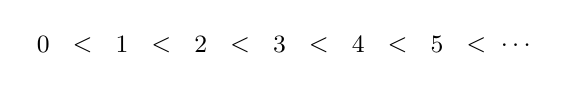
\begin{tikzpicture}
	\foreach \x/\xtext in {0, 1, 2, 3, 4, 5}
	{
		\node (\x a) at (\x, 1) {\small{$\x$}};
		\node (\x a) at (\x.5, 1) {\small{$<$}};
	}
	\node (ldots) at (6, 1) {\small{$\ldots$}};
	\end{tikzpicture}
\end{center}
We call this, in the jargon, an $\omega$-sequence. And indeed, this
general ordering is mirrored in our initial construction of the stages
of the set hierarchy. But, now suppose we move $0$ to the end of this
sequence, so that it comes after all the other numbers:
\begin{center}
	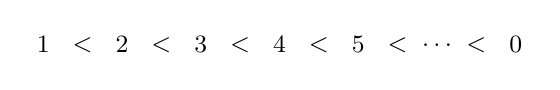
\begin{tikzpicture}
	\foreach \x/\xtext in {1, 2, 3, 4, 5}
	{
		\node (\x a) at (\x, 1) {\small{$\x$}};
		\node (\x a) at (\x.5, 1) {\small{$<$}};
	}
	\node (ldots) at (6, 1) {\small{$\ldots$}};
	\node (bea) at (6.5, 1) {\small{$<$}};
	\node (noa) at (7, 1) {\small{$0$}};
	\end{tikzpicture}
\end{center}
We have the same entities here, but ordered in a fundamentally
different way: our first ordering had no last element; our new
ordering does. Indeed, our new ordering consists of an
$\omega$-sequence of entities ($1, 2, 3, 4, 5, \ldots$), followed by
another entity. It will be an $\omega+1$-sequence.

We can generate even more types of ordering, using just these
entities. For example, consider all the even numbers (in their natural
order) followed by all the odd numbers (in their natural order):
\begin{center}
	\begin{tikzpicture}
	\node(a1) at (1,1) {\small{$0$}};
	\node(a2) at (1.5,1) {\small{$<$}};
	\node(a3) at (2,1) {\small{$2$}};
	\node(a4) at (2.5,1) {\small{$<$}};
	\node(a5) at (3,1) {\small{$4$}};
	\node(a6) at (3.5,1) {\small{$<$}};
	\node(dots) at (4,1) {\small{$\ldots$}};
	\node(aaoe) at (4.5,1) {\small{$<$}};
	\node(b1) at (5,1) {\small{$1$}};
	\node(b2) at (5.5,1) {\small{$<$}};
	\node(b3) at (6,1) {\small{$3$}};
	\node(b4) at (6.5,1) {\small{$<$}};
	\node(b5) at (7,1) {\small{$\ldots$}};
	\end{tikzpicture}
\end{center}
This is an $\omega$-sequence followed by another $\omega$-sequence; an
$\omega+\omega$-sequence. 

Well, we can keep going. But what we would like is a general way to
understand this talk about \emph{orderings}. 

% ==== OLP file: content/set-theory/ordinals/introduction.tex ====
% Part: set-theory
% Chapter: ordinals
% Section: introduction



\olfileid{sth}{ordinals}{intro}

\olsection{Introduction}

In \olref[z][]{chap}, we postulated that there is an infinite-th stage
of the hierarchy, in the form of \stagesinf{} (see also our axiom of
Infinity). However, given \stagessucc{}, we can't stop at the
infinite-th stage; we have to keep going. So: at the next stage after
the first infinite stage, we form all possible collections of sets
that were available at the first infinite stage; and repeat; and
repeat; and repeat; \dots

Implicitly what has happened here is that we have started to invoke an
``intuitive'' notion of number, according to which there can be
numbers \emph{after} all the natural numbers. In particular, the
notion involved is that of a \emph{transfinite ordinal}. The aim of
this chapter is to make this idea more rigorous. We will explore the
general notion of an ordinal, and then explicitly define certain sets
to be our ordinals. 

% ==== OLP file: content/set-theory/ordinals/iso.tex ====


\olfileid{sth}{ordinals}{iso}
\olsection{Order-Isomorphisms}

To explain \emph{how} robust well-ordering is, we will start by
introducing a method for comparing well-orderings.

\begin{defn}
A \emph{well-ordering} is a pair $\tuple{A, <}$, such that $<$
well-orders $A$. The well-orderings $\tuple{A, <}$ and $\tuple{B,
\lessdot}$ are \emph{order-isomorphic} {iff} there is !!a{bijection}
$f \colon A \to B$ such that: $x < y$ iff $f(x) \lessdot  f(y)$. In
this case, we write $\ordeq{\tuple{A, <}}{\tuple{B, \lessdot}}$, and
say that $f$ is an \emph{order-isomorphism}.
\end{defn}
\noindent
In what follows, for brevity, we will speak of ``isomorphisms'' rather
than ``order-isomorphisms''. Intuitively, isomorphisms are
structure-preserving !!{bijection}s. Here are some simple facts about
isomorphisms.

\begin{lem}\ollabel{isoscompose}
Compositions of isomorphisms are isomorphisms, i.e.: if $f \colon A
\to B$ and $g \colon B \to C$ are isomorphisms, then $(g \circ f)
\colon A \to C$ is an isomorphism.
\end{lem}
\begin{prob}
	Prove \olref[sth][ordinals][iso]{isoscompose}.
\end{prob}
\begin{proof}
Left as an exercise.
\end{proof}
\begin{cor}\ollabel{ordisoisequiv}
	$\ordeq{X}{Y}$ is an equivalence relation.
\end{cor}
\begin{prop}\ollabel{ordisounique}
If $\tuple{A, <}$ and $\tuple{B, \lessdot}$ are isomorphic
well-orderings, then the isomorphism between them is unique.
\end{prop}

\begin{proof}
Let $f$ and $g$ be isomorphisms $A \to B$. We will prove the result by induction, i.e.\ using \olref[wo]{propwoinduction}. 
Fix $a\in A$, and suppose (for induction) that $(\forall b < a)f(b) = g(b)$. Fix $x \in B$. 

If $x \lessdot f(a)$, then $f^{-1}(x) < a$, so $g(f^{-1}(x)) \lessdot
g(a)$, invoking the fact that $f$ and $g$ are isomorphisms. But since
$f^{-1}(x) < a$, by our supposition $x =f(f^{-1}(x)) = g(f^{-1}(x))$.
So $x \lessdot g(a)$. Similarly, if $x \lessdot g(a)$ then $x \lessdot
f(a)$. 

Generalising, $(\forall x \in B)(x \lessdot f(a) \liff x \lessdot
g(a))$. It follows that $f(a) = g(a)$ by
\olref[sfr][rel][ord]{prop:extensionality-strictlinearorders}. So $(\forall
a \in A)f(a) = g(a)$ by \olref[wo]{propwoinduction}.
\end{proof}\noindent 
This gives some sense that well-orderings are robust. But to continue
explaining this, it will help to introduce some more notation. 

\begin{defn}
When $\tuple{A, <}$ is a well-ordering with $a \in A$, let $A_a = \Setabs{x \in A}{x
< a}$. We say that $A_a$ is a proper \emph{initial segment} of $A$ (and allow that $A$ itself is an improper initial segment of $A$). Let
$<_a$ be the restriction of $<$ to the initial segment, i.e.,
$\funrestrictionto{\mathord{<}}{A_a^2}$. 
\end{defn}
\noindent
Using this notation, we can state and prove that no well-ordering is
isomorphic to any of its proper initial segments.

\begin{lem}\ollabel{wellordnotinitial}
If $\tuple{A, <}$ is a well-ordering with $a \in A$, then
$\ordneq{\tuple{A, <}}{\tuple{A_a, <_a}}$ 
\end{lem}

\begin{proof}
For reductio, suppose $f \colon A \to A_a$ is an isomorphism. Since
$f$ is a bijection and $A_a \subsetneq A$, using \olref[wo]{wo:strictorder} let $b \in A$ be the
$<$-least !!{element} of $A$ such that $b \neq f(b)$. We'll show that
$(\forall x \in A)(x<b \liff x < f(b))$, from which it will follow by
\olref[sfr][rel][ord]{prop:extensionality-strictlinearorders} that $b =
f(b)$, completing the reductio.

Suppose $x < b$. So $x = f(x)$, by the choice of $b$. And $f(x) <
f(b)$, as $f$ is an isomorphism. So $x < f(b)$.

Suppose $x < f(b)$. So $f^{-1}(x) < b$, since $f$ is an isomorphism,
and so $f^{-1}(x) = x$ by the choice of $b$. So $x < b$. 
\end{proof}

Our next result shows, roughly put, that an ``initial segment'' of an
isomorphism is an isomorphism:

\begin{lem}\ollabel{wellordinitialsegment}
Let $\tuple{A, <}$ and $\tuple{B, \lessdot}$ be well-orderings. If $f
\colon A \to B$ is an isomorphism and $a \in A$, then
$\funrestrictionto{f}{A_{a}} : A_a \to B_{f(a)}$ is an isomorphism.
\end{lem}

\begin{proof}
Since $f$ is an isomorphism:
	%Since $f$ is an isomorphism, $b < a$ iff $f(b) \lessdot f(a)$, so that 
\begin{align*}
	\funimage{f}{A_a} &= \funimage{f}{\Setabs{x \in A}{x < a}}\\
	&= \funimage{f}{\Setabs{f^{-1}(y) \in A}{f^{-1}(y) < a}} \\
	&= \Setabs{y \in B}{y \lessdot f(a)} \\
	&=B_{f(a)} 
\end{align*}
And $\funrestrictionto{f}{A_a}$ preserves order because $f$ does. 
\end{proof}

Our next two results establish that well-orderings are always
comparable:

\begin{lem}\ollabel{lemordsegments}
Let $\tuple{A, <}$ and $\tuple{B, \lessdot}$ be well-orderings. If
$\ordeq{\tuple{A_{a_1}, <_{a_1}}}{\tuple{B_{b_1}, \lessdot_{b_1}}}$
and $\ordeq{\tuple{A_{{a_2}}, <_{a_2}}}{\tuple{B_{{b_2}},
\lessdot_{b_2}}}$, then ${a_1}  < {a_2} \text{ iff }{b_1} \lessdot
{b_2}$
\end{lem}

\begin{proof}
We will prove \emph{left to right}; the other direction is similar.
Suppose both $\ordeq{\tuple{A_{a_1}, <_{a_1}}}{\tuple{B_{b_1},
\lessdot_{b_1}}}$ and $\ordeq{\tuple{A_{{a_2}},
<_{a_2}}}{\tuple{B_{{b_2}}, \lessdot_{b_2}}}$, with $f \colon
A_{{a_2}} \to B_{{b_2}}$ our isomorphism. Let ${a_1} < {a_2}$; then
$\ordeq{\tuple{A_{a_1}, <_{a_1}}}{\tuple{B_{f({a_1})},
\lessdot_{f({a_1})}}}$ by \olref{wellordinitialsegment}. So
$\ordeq{\tuple{B_{b_1}, \lessdot_{b_1}}}{\tuple{B_{f({a_1})},
\lessdot_{f({a_1})}}}$, and so ${b_1} = f({a_1})$ by
\olref{wellordnotinitial}. Now ${b_1} \lessdot {b_2}$ as $f$'s domain
is $B_{{b_2}}$.	
\end{proof}

\begin{thm}\ollabel{thm:woalwayscomparable}
Given any two well-orderings, one is isomorphic to an initial segment
(not necessarily proper) of the other.
\end{thm}

\begin{proof}
Let $\tuple{A, <}$ and $\tuple{B, \lessdot}$ be well-orderings. Using
Separation, let
\[
	f = \Setabs{\tuple{a, b} \in A \times B}{
		\ordeq{\tuple{A_a, <_a}}{\tuple{B_b, \lessdot_b}}}.
\]
By \olref{lemordsegments}, $a_1 < a_2$ iff $b_1 \lessdot b_2$ for all
$\tuple{a_1, b_1}, \tuple{a_2, b_2} \in f$. So $f \colon \dom{f} \to
\ran{f}$ is an isomorphism. 

If $a_2 \in \dom{f}$ and $a_1 < a_2$, then $a_1 \in \dom{f}$ by
\olref{wellordinitialsegment}; so $\dom{f}$ is an initial segment of
$A$. Similarly, $\ran{f}$ is an initial segment of $B$. For reductio,
suppose both are \emph{proper} initial segments. Then let $a$ be the
$<$-least !!{element} of $A \setminus \dom{f}$, so that $\dom{f} =
A_a$, and let $b$ be the $\lessdot$-least !!{element} of $B \setminus
\ran{f}$, so that $\ran{f} = B_b$. So $f \colon A_a \to B_b$ is an
isomorphism, and hence $\tuple{a, b} \in f$, a contradiction.
\end{proof}


% ==== OLP file: content/set-theory/ordinals/milestone.tex ====

\olfileid{sth}{ordinals}{zfm}	
\olsection{$\ZFminus$: a milestone}

The question of how to justify Replacement (if at all) is not
straightforward. As such, we will reserve that for
\olref[replacement][]{chap}. However, with the addition of Replacement, we
have reached another important milestone. We now have all the axioms
required for the theory $\ZFminus$. In detail:

\begin{defn}
The theory $\ZFminus$ has these axioms: Extensionality, Union, Pairs,
Powersets, Infinity, and all instances of the Separation and
Replacement schemes. Otherwise put, $\ZFminus$ adds Replacement to
$\Zminus$.
\end{defn}
\noindent
This stands for \emph{Zermelo--Fraenkel} set theory (\emph{minus}
something which we will come to later). Fraenkel gets the honour,
since he is credited with the formulation of Replacement in
\citeyear{Fraenkel1922}, although the first precise formulation was
due to \citet{Skolem1922}.

% ==== OLP file: content/set-theory/ordinals/opps.tex ====


\olfileid{sth}{ordinals}{opps}
\olsection{Successor and Limit Ordinals}

In the next few chapters, we will use ordinals a great deal. So it
will help if we introduce some simple notions. 

\begin{defn}
For any ordinal $\alpha$, its \emph{successor} is $\ordsucc{\alpha}
=\alpha \cup \{\alpha\}$. We say that $\alpha$ is a \emph{successor}
ordinal if $\ordsucc{\beta} = \alpha$ for some ordinal~$\beta$. We
say that $\alpha$ is a \emph{limit} ordinal iff $\alpha$ is neither
empty nor a successor ordinal.
\end{defn}
\noindent
The following result shows that this is the right notion of
\emph{successor}:

\begin{prop}
For any ordinal $\alpha$:
\begin{enumerate}
	\item $\alpha \in \ordsucc{\alpha}$;
	\item $\ordsucc{\alpha}$ is an ordinal;
	\item there is no ordinal $\beta$ such that $\alpha \in \beta \in
	\ordsucc{\alpha}$.
	\end{enumerate}
\end{prop}

\begin{proof}
Trivially, $\alpha \in \alpha \cup \{\alpha\} = \ordsucc{\alpha}$.
Equally, $\ordsucc{\alpha}$ is a transitive set of ordinals, and hence
an ordinal by \olref[basic]{corordtransitiveord}.
And it is impossible that $\alpha \in \beta \in \ordsucc{\alpha}$,
since then either $\beta \in \alpha$ or $\beta = \alpha$,
contradicting \olref[basic]{ordordered}.
\end{proof}
\noindent
This also licenses a variant of proof by transfinite induction:

\begin{thm}[Simple Transfinite Induction]\ollabel{simpletransrecursion}
Let $\phi(x)$ be a formula such that:
\begin{enumerate}
	\item $\phi(\emptyset)$; and
	\item for any ordinal $\alpha$, if $\phi(\alpha)$ then
	$\phi(\ordsucc{\alpha})$; and 
	\item if $\alpha$ is a limit ordinal and $(\forall \beta \in
	\alpha)\phi(\beta)$, then $\phi(\alpha)$.
\end{enumerate}
Then $\forall \alpha \phi(\alpha)$.
\end{thm}

\begin{proof}
We prove the contrapositive. So, suppose there is some ordinal which
is $\lnot\phi$; let $\gamma$ be the least such ordinal. Then either
$\gamma = \emptyset$, or $\gamma = \ordsucc{\alpha}$ for some $\alpha$
such that $\phi(\alpha)$; or $\gamma$ is a limit ordinal and $(\forall
\beta \in \gamma)\phi(\beta)$.
\end{proof}
\noindent
A final bit of notation will prove helpful later on:

\begin{defn}\ollabel{defsupstrict}
If $X$ is a  set of ordinals, then $\supstrict(X) = \bigcup_{\alpha
\in X} \ordsucc{\alpha}$.
\end{defn}
\noindent
Here, ``lsub'' stands for ``least strict upper bound''.\footnote{Some
books use ``$\text{sup}(X)$'' for this.  But other books use
``$\text{sup}(X)$'' for the least \emph{non-strict} upper bound, i.e.,
simply $\bigcup X$. If $X$ has a greatest element, $\alpha$, these
notions come apart: the least \emph{strict} upper bound is
$\ordsucc{\alpha}$, whereas the least \emph{non-strict} upper bound is
just $\alpha$.}  The following result explains this:

\begin{prop}
If $X$ is a set of ordinals, $\supstrict(X)$ is the least ordinal
greater than every ordinal in $X$.
\end{prop}

\begin{proof}
Let $Y = \Setabs{\ordsucc{\alpha}}{\alpha \in X}$, so that
$\supstrict(X) = \bigcup Y$. Since ordinals are transitive and every
member of an ordinal is an ordinal, $\supstrict(X)$ is a transitive
set of ordinals, and so is an ordinal by
\olref[basic]{corordtransitiveord}. 

If $\alpha \in X$, then $\ordsucc{\alpha} \in Y$, so $\ordsucc{\alpha}
\subseteq \bigcup Y = \supstrict(X)$, and hence $\alpha \in
\supstrict(X)$. So $\supstrict(X)$ is strictly greater than every
ordinal in $X$.

Conversely, if $\alpha \in \supstrict(X)$, then $\alpha \in
\ordsucc{\beta} \in Y$ for some $\beta \in X$, so that $\alpha \leq
\beta \in X$. So $\supstrict(X)$ is the \emph{least} strict upper
bound on $X$.
\end{proof}

% ==== OLP file: content/set-theory/ordinals/ordinals.tex ====
% Chapter: Naive



\olchapter{sth}{ordinals}{Ordinals}

\olimport{introduction}
\olimport{idea}
\olimport{wo}
\olimport{iso}
\olimport{vn}
\olimport{basic}
\olimport{replacement}
\olimport{milestone}
\olimport{ordtype}
\olimport{opps}

\OLEndChapterHook

% ==== OLP file: content/set-theory/ordinals/ordtype.tex ====


\olfileid{sth}{ordinals}{ordtype}
\olsection{Ordinals as Order-Types}

Armed with Replacement, and so now working in $\ZFminus$, we can finally prove the result we have been aiming for:

\begin{thm}\ollabel{thmOrdinalRepresentation}
Every well-ordering is isomorphic to a unique ordinal. 
\end{thm}

\begin{proof}
Let $\tuple{A, <}$ be a well-order. By
\olref[basic]{ordisoidentity}, it is isomorphic to at most one
ordinal. So, for reductio, suppose $\tuple{A, <}$ is not isomorphic to
\emph{any} ordinal. We will first ``make $\tuple{A, <}$ as small as
possible''. In detail: if some proper initial segment $\tuple{A_a,
<_a}$ is not isomorphic to any ordinal, there is a least $a \in A$
with that property; then let $B = A_a$ and $\mathord{\lessdot} =
\mathord{<_a}$. Otherwise, let $B = A$ and $\mathord{\lessdot} =
\mathord{<}$. 

By definition, every proper initial segment of $B$ is isomorphic to
some ordinal, which is unique as above. So
by Replacement, the following set exists, and is a function:
\[
	f = \Setabs{\tuple{\beta, b}}{b \in B\text{ and }\ordeq{\beta}{\tuple{B_b, \lessdot_b}}}
\]
To complete the reductio, we'll show that $f$ is an isomorphism
$\alpha \to B$, for some ordinal $\alpha$. 

It is obvious that $\ran{f}
= B$. And by \olref[iso]{lemordsegments}, $f$ preserves ordering,
i.e., $\gamma \in \beta$ iff $f(\gamma) \lessdot f(\beta)$. To show that $\dom{f}$ is an ordinal, by
\olref[basic]{corordtransitiveord} it suffices to show that
$\dom{f}$ is transitive. So fix $\beta \in \dom{f}$, i.e.,
$\ordeq{\beta}{\tuple{B_b, \lessdot_b}}$ for some $b$. If $\gamma \in
\beta$, then $\gamma \in \dom{f}$ by
\olref[iso]{wellordinitialsegment}; generalising, $\beta \subseteq
\dom{f}$.
\end{proof}

This result licenses the following definition, which we have wanted to
offer since \olref[vn]{sec}:

\begin{defn}
If $\tuple{A, <}$ is a well-ordering, then its order type,
$\ordtype{A, <}$, is the unique ordinal $\alpha$ such that
$\ordeq{\tuple{A, < }}{\alpha}$.
\end{defn}

Moreover, this definition licenses two nice principles:

\begin{cor}\ollabel{ordtypesworklikeyouwant}
Where $\tuple{A, <}$ and $\tuple{B, \lessdot}$ are well-orderings: 
\begin{align*}
	\ordtype{A, <} = \ordtype{B, \lessdot}&\text{ iff }\ordeq{\tuple{A, <}}{\tuple{B, \lessdot}}\\
	\ordtype{A, <} \in \ordtype{B, \lessdot}&\text{ iff }\ordeq{\tuple{A, <}}{\tuple{B_b, \lessdot_b}}\text{ for some }b \in B
\end{align*}
\end{cor}

\begin{proof}
The identity holds by \olref[basic]{ordisoidentity}. To prove
the second claim, let $\ordtype{A, <} = \alpha$ and $\ordtype{B,
\lessdot} = \beta$, and let $f \colon \beta \to \tuple {B, \lessdot}$
be our isomorphism. Then:
\begin{align*}
	\alpha \in \beta&\text{ iff }\funrestrictionto{f}{\alpha} \colon \alpha \to B_{f(\alpha)}\text{ is an isomorphism}\\
	&\text{ iff }\ordeq{\tuple{A, <}}{\tuple{B_{f(\alpha)}, \lessdot_{f(\alpha)}}}\\
	&\text{ iff }\ordeq{\tuple{A, <}}{\tuple{B_b, \lessdot_b}}\text{ for some $b \in B$}
\end{align*}
by \olref[iso]{ordisounique},
\olref[iso]{wellordinitialsegment}, and
\olref[basic]{ordissetofsmallerord}.
\end{proof}

% ==== OLP file: content/set-theory/ordinals/replacement.tex ====


\olfileid{sth}{ordinals}{replacement}
\olsection{Replacement}

In \olref[sth][ordinals][vn]{sec}, we motivated the introduction of ordinals by
suggesting that we could treat them as order-types, i.e., canonical
proxies for well-orderings. In order for that to work, we would need
to prove that \emph{every well-ordering is isomorphic to some
ordinal}. This would allow us to define $\ordtype{A, <}$ as the
ordinal $\alpha$ such that $\tuple{A, <} \isomorphic \alpha$. 

Unfortunately, we \emph{cannot} prove the desired result only the
Axioms we provided introduced so far. (We will see why in
\olref[replacement][strength]{sec}, but for now the point is: we can't.) We need a
new thought, and here it is:

\begin{axiom}[Scheme of Replacement]
For any formula $\phi(x, y)$, the following is an axiom:
\begin{quote}
	for any $A$, if $(\forall x \in A)\lexists![y][\phi(x,y)]$, then
	$\Setabs{y}{(\exists x \in A)\phi(x,y)}$ exists.
\end{quote}
\end{axiom}
\noindent
As with Separation, this is a scheme: it yields infinitely many
axioms, for each of the infinitely many different $\phi$'s. And it can
equally well be (and normally is) written down thus:

\begin{defish}
For any formula $\phi(x,y)$ which does not contain ``$B$'', the following is an axiom:
\[
\forall A[(\forall x \in A)\lexists![y][\phi(x,y)] \lif \exists B\forall y (y \in B \liff (\exists x \in A)\phi(x,y))]
\]
\end{defish}

On first encounter, however, this is quite a tangled formula. The
following quick consequence of Replacement probably gives a
\emph{clearer} expression to the intuitive idea we are working with:\footnote{A term is an expression which picks out exactly one object (on any completion of its free variables). For example, ``$\emptyset$'' is a term which picks out the empty set; ``$\{x\}$'' is a term which picks out $x$'s singleton (whatever $x$ might be); ``$x \cup y$'' is a term which picks out the union of $x$ and $y$ (whatever they might be).}

\begin{cor}
For any term $\tau(x)$, and any set $A$, this set exists:
\[
	\Setabs{\tau(x)}{x \in A} = \Setabs{y}{(\exists x \in A)y = \tau(x)}.
\]
\end{cor}

\begin{proof}
Since $\tau$ is a \emph{term}, $\forall x \lexists![y][\tau(x) = y]$.
A fortiori, $(\forall x \in A)\lexists![y][\tau(x) = y]$. So
$\Setabs{y}{(\exists x \in A)\tau(x) = y}$ exists by Replacement.
\end{proof}
\noindent
This suggests that ``Replacement'' is a good name for the Axiom: given
a set $A$, you can form a new set, $\Setabs{\tau(x)}{x \in A}$, by
replacing every member of $A$ with its image under~$\tau$. Indeed,
following the notation for the image of a set under a function, we
might write $\funimage{\tau}{A}$ for $\Setabs{\tau(x)}{x \in A}$.

Crucially, however, $\tau$ is a \emph{term}. It need not be (a name
for) a \emph{function}, in the sense of \olref[sfr][fun][rel]{sec},
i.e., a certain set of ordered pairs. After all, if $f$ is a function
(in that sense), then the set $\funimage{f}{A} = \Setabs{f(x)}{x \in
A}$ is just a particular subset of $\ran{f}$, and that is already
guaranteed to exist, just using the axioms of~$\Zminus$.\footnote{Just
consider $\Setabs{y \in \bigcup \bigcup f}{(\exists x \in A)y =
f(x)}$.} Replacement, by contrast, is a \emph{powerful} addition to
our axioms, as we will see in \olref[sth][replacement][]{chap}.



% ==== OLP file: content/set-theory/ordinals/vn.tex ====


\olfileid{sth}{ordinals}{vn}	
\olsection[Von Neumann's Construction]{Von Neumann's Construction of the Ordinals}

\olref[sth][ordinals][iso]{thm:woalwayscomparable} gives rise to a
thought. We could introduce certain objects, called \emph{order
types}, to go proxy for the well-orderings. Writing $\ordtype{A, <}$
for the order type of the well-ordering $\tuple{A, <}$, we would hope
to secure the following two principles:
\begin{align*}
	\ordtype{A, <} = \ordtype{B, \lessdot} & 
	\text{ iff } \ordeq{\tuple{A, <}}{\tuple{B, \lessdot}}\\
	\ordtype{A, <} < \ordtype{B, \lessdot}&
	\text{ iff }\ordeq{\tuple{A, <}}{\tuple{B_b, \lessdot_b}}\text{ for some }b \in B
\end{align*}
Moreover, we might hope to introduce order-types \emph{as certain
sets}, just as we can introduce the natural numbers as certain sets. 

The most common way to do this---and the approach we will follow---is
to define these order-types via certain \emph{canonical} well-ordered
sets. These canonical sets were first introduced by von Neumann:

\begin{defn}
The set $A$ is \emph{transitive} {iff} $(\forall x \in A)x \subseteq
A$. Then $A$ is an \emph{ordinal} {iff} $A$ is transitive and
well-ordered by $\in$.
\end{defn}
\noindent
In what follows, we will use Greek letters for ordinals. It follows
immediately from the definition that, if $\alpha$ is an ordinal, then
$\tuple{\alpha, \in_\alpha}$ is a well-ordering, where $\in_\alpha =
\Setabs{\tuple{x, y} \in \alpha^2}{x \in y}$. So, abusing notation a
little, we can just say that $\alpha$ \emph{itself} is a
well-ordering. 

Here are our first few ordinals:
\[
	\emptyset, \{\emptyset\}, 
	\{\emptyset, \{\emptyset\}\}, 
	\{\emptyset, \{\emptyset\}, \{\emptyset, \{\emptyset\}\}\}, \ldots
\]
You will note that these are the first few ordinals that we
encountered in our Axiom of Infinity, i.e., in von Neumann's
definition of $\omega$ (see \olref[sth][z][infinity-again]{sec}). This
is no coincidence. Von Neumann's definition of the ordinals treats
natural numbers as ordinals, but allows for transfinite ordinals too. 

As always, we can now ask: \emph{are} these the ordinals? Or has von
Neumann simply given us some sets that we can \emph{treat} as the
ordinals? The kinds of discussions one might have about this question
are similar to the discussions we had in \olref[sfr][rel][ref]{sec},
\olref[sfr][arith][ref]{sec},
\olref[sfr][infinite][dedekindsproof]{sec}, and
\olref[sth][z][nat]{sec}, so we will not belabour the point.
Instead, in what follows, we will simply use ``the ordinals'' to speak
of ``the von Neumann ordinals''. 

% ==== OLP file: content/set-theory/ordinals/wo.tex ====


\olfileid{sth}{ordinals}{wo}
\olsection{Well-Orderings}

The fundamental notion is as follows:

\begin{defn}
The relation $<$ \emph{well-orders} $A$ iff it meets these two conditions:
\begin{enumerate}
	\item $<$ is connected, i.e., for all $a, b \in A$, either $a < b$
	or $a = b$ or $b < a$;
	\item every non-empty subset of $A$ has a $<$-minimal !!{element},
	i.e., if $\emptyset \neq X \subseteq A$ then $(\exists m \in
	X)(\forall z \in X)z \nless m$
\end{enumerate}
\end{defn}

It is easy to see that three examples we just considered were indeed
well-ordering relations. 

\begin{prob}
\Olref[sth][ordinals][idea]{sec} presented three example orderings
on the natural numbers. Check that each is a well-ordering.
\end{prob}

Here are some elementary but extremely important observations
concerning well-ordering.

\begin{prop}\ollabel{wo:strictorder}
If $<$ well-orders $A$, then every non-empty subset of $A$ has a unique
$<$-least member, and $<$ is irreflexive, asymmetric and transitive.
\end{prop}

\begin{proof}
If $X$ is a non-empty subset of $A$, it has a $<$-minimal !!{element}
$m$, i.e., $(\forall z \in X)z \nless m$. Since $<$ is connected,
$(\forall z \in X)m \leq z$. So $m$ is the $<$-least !!{element} of $X$.

For irreflexivity, fix $a \in A$; the $<$-least !!{element} of $\{a\}$ is $a$, so $a \nless a$. For transitivity, if $a < b < c$, then
since $\{a, b, c\}$ has a $<$-least !!{element}, $a < c$. Asymmetry
follows from irreflexivity and transitivity
\end{proof}

\begin{prop}\ollabel{propwoinduction}
If $<$ well-orders $A$, then for any formula $\phi(x)$:
\[
	\text{if }(\forall a \in A)((\forall b < a)\phi(b) \lif 
		\phi(a))\text{, then }(\forall a \in A)\phi(a).
\]
\end{prop}

\begin{proof}
We will prove the contrapositive. Suppose $\lnot(\forall a \in
A)\phi(a)$, i.e., that $X = \Setabs{x \in A}{\lnot\phi(x)} \neq
\emptyset$. Then $X$ has an $<$-minimal !!{element}, $a$. So $(\forall
b < a)\phi(b)$ but $\lnot \phi(a)$. \end{proof}\noindent This last
property should remind you of the principle of strong induction on the
naturals, i.e.: if $(\forall n \in \omega)((\forall m < n)\phi(m)
\lif \phi(n))$, then $(\forall n \in \omega)\phi(n)$. And this
property makes well-ordering into a very \emph{robust} notion.\footnote{A reminder: all formulas can have parameters (unless explicitly stated otherwise).} 

